% !TEX root = ../thesis.tex
%
\chapter{Preliminary Studies}
\label{sec:preliminary}

In order to determine the usability of Ohua for implementeing shared state applications and to identify any necessary modifications to the compiler or the runtime, we first tried to implement a single such application in Ohua.
After successful implementation we wanted tocompare its performance against a STm implementation of the same program and see, whether there are any shortcomings of Ohua in terms of performance.
Based on this initial study we then wanted to find ways to improve Ohua's performance, if necessary, e.g. by introducing new compiler optimizations.
The aim of these preliminary studies was to find out, whether Ohua was usable for writing programs relying on shared state and if it could be a viable alternative to STM in this setting.

\section{Labyrinth Benchmark}

As a first example application, we chose to implement the \emph{labyrinth} benchmark as presented by Swalens et al.~\cite{swalens2016transactional}.
This algorithm is a variation of Lee's Algorithm~\cite{lee1961algorithm} which solves path-connection problems often encountered when searching for an optimal route or generating wiring diagrams where wires may not overlap.
We base our own implementation on the descriptions of Watson et al.~\cite{watson2007study}, who presented an implementation for Transactional Memory.

\begin{figure}[b]
    \begin{subfigure}[t]{.24\textwidth}
        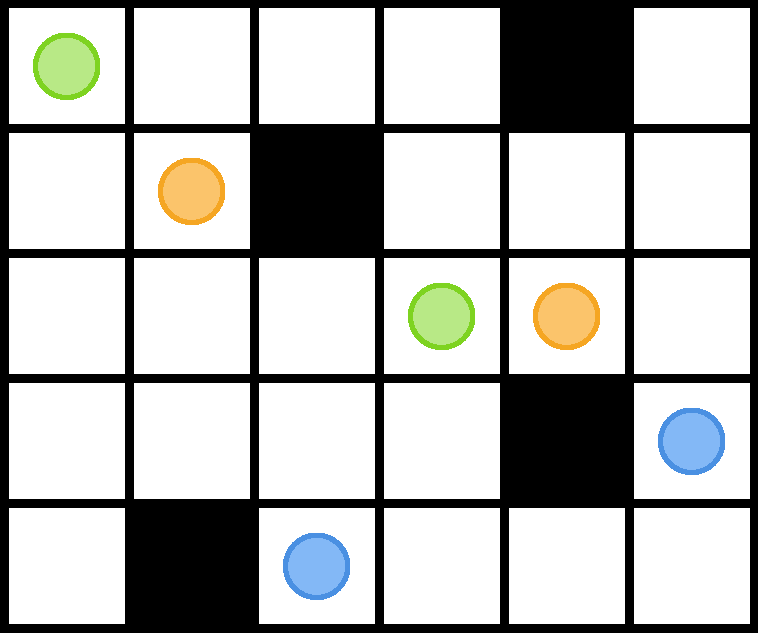
\includegraphics[width=\textwidth,keepaspectratio]{gfx/preliminaries-labyrinth/1-maze_points}
        \caption{Initial grid with 3 point pairs.}%
    \end{subfigure}%
    ~
    \begin{subfigure}[t]{.24\textwidth}
        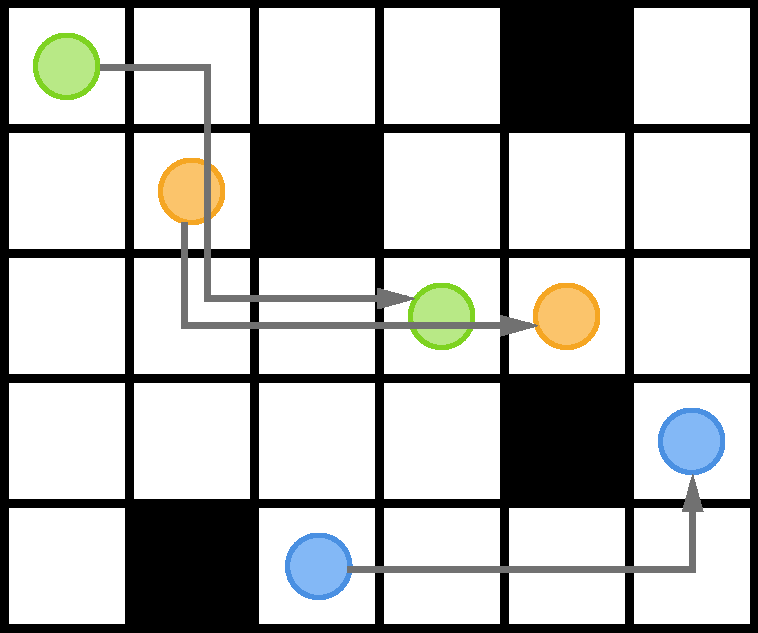
\includegraphics[width=\textwidth,keepaspectratio]{gfx/preliminaries-labyrinth/2-maze_paths}
        \caption{Possible paths between the points.}%
    \end{subfigure}%
    ~
    \begin{subfigure}[t]{.24\textwidth}
        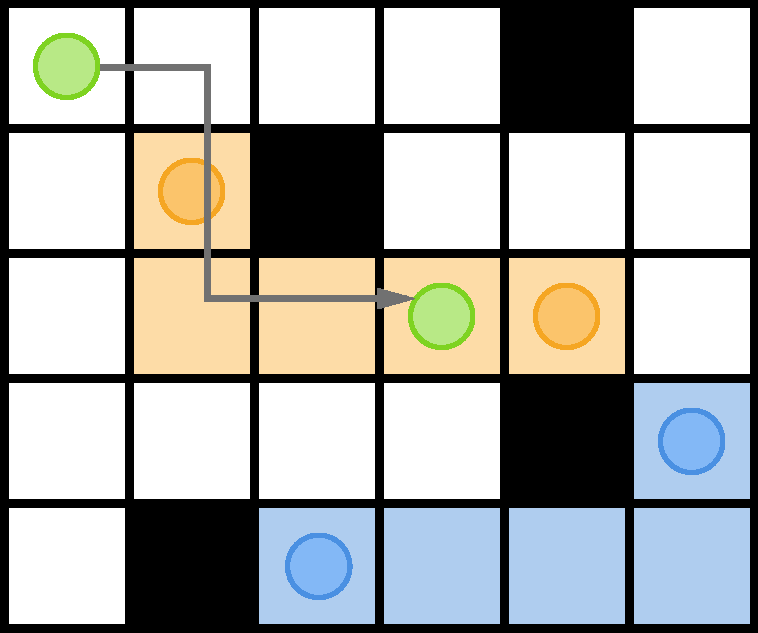
\includegraphics[width=\textwidth,keepaspectratio]{gfx/preliminaries-labyrinth/4-maze_update2}
        \caption{First two paths are mapped into the maze.}%
    \end{subfigure}%
    ~
    \begin{subfigure}[t]{.24\textwidth}
        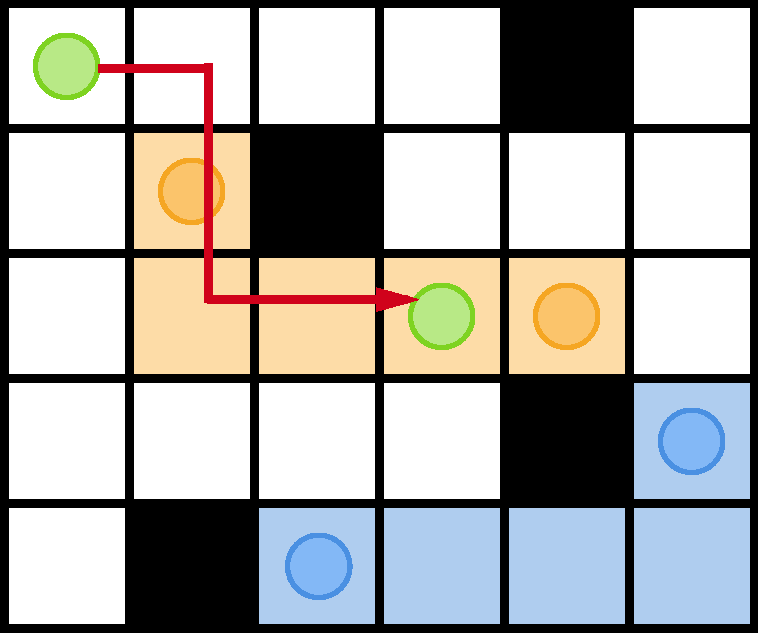
\includegraphics[width=\textwidth,keepaspectratio]{gfx/preliminaries-labyrinth/5-maze_update3}
        \caption{Conflict for the third path as it goes through a now-occupied segment.}%
        \label{fig:preliminary:labyrinth:unroutable}
    \end{subfigure}%
    \caption{Illustration of the operation of the labyrinth benchmark, showing the (attempted) mapping of 3 paths in a 6 $\times$ 5 two-dimensional grid. Black squares represent walls that cannot be routed through.}%
    \label{fig:preliminary:labyrinth}
\end{figure}

Goal of the benchmark is to find a number of paths within a three-dimensional maze, as depicted in Fig.~\ref{fig:preliminary:labyrinth}.
As input, the algorithm is provided with a maze and a set of pairs of points, between which a path is to be found and mapped within the maze.
During execution, one pair of coordinates is removed from the list of points (the worklist) and the program attempts to find a path between both points in the maze.
This is done using a breadth-first search.
The maze itself may also contain \enquote{walls} (highlighted as black squares in Fig.~\ref{fig:preliminary:labyrinth}), through which no path can be routed.
Also, each point in the maze may only occupied by a single path to rule out overlapping paths.
The algorithm terminates once the worklist is empty and all paths have either been mapped successfully or deemed unmappable by the absence of a valid connection between both points.

This benchmark is a classic example for an \emph{irregular application}: all operations happen on the shared maze data structure which is modified in the process.
Additionally, any data parallelism obtainable in the application is \emph{amorphous}, as mapping one path in the maze may render another pair of coordinates unroutable as both points get cut off from one another.
An example for this can be seen in Fig.~\ref{fig:preliminary:labyrinth:unroutable}, where the mapping of the orange path makes finding a path between the green coordinates impossible as one point is part of the orange path.
As we have learned in chapter~\ref{sec:background:irregular}, this specific class of problems can be parallelized easily using Software Transactional Memory.
Searching for a single path could be compartmented into a transaction, treating all maze fields as transaction variables.
Listing~\ref{fig:preliminaries:stm} shows the resultimg transactional implementation of the labyrinth benchmark.

\begin{figure}[t]
    \begin{minted}{Rust}
        let (worklist, grid) = /* read from file */

        for points in worklist {
            atomically(|trans| {
                let local_grid = create_working_copy(&grid);

                if let Some(path) = find_path(points, &local_grid) {
                    // if path is found, write back results
                    update_grid(&grid, &path, trans)?;
                }

                Ok(())
            });
        }
    \end{minted}
    \caption{Simple implementation of the labyrinth benchmarks using Software Transactional Memory}%
    \label{fig:preliminaries:stm}
\end{figure}

All path pairs are collected in a worklist, through which the algorithm iterates (line 3).
Inside the transaction that is started for each item (line 4), a working copy of the maze is created as detailed in~\cite{swalens2016transactional} to reduce the number of repeated reads from individual transaction variables.
Then, the breadth-first search commences in order to discover a route between the starting point and the target (line 7).
Note that since we've made a copy of the grid beforehand, this happens completely locally.
When a path is found, an update is run on the grid, inserting the path (line 9).
Should another transaction, which also happened to alter one or more segments of the newly-found path, manage to commit in the meantime, the resulting conflict is detected and the transaction is rolled back and re-run until either the update commits successfully or no path can be found anymore.
Our transactional memory implementation is a mere adaption of the algorithm outlined above, augmented with concurrency by splitting the worklist into $n$ parts, which are processed by $n$ threads in parallel.

In our first Ohua implementation, we described idiomatically, what the algorithm should be doing.
Fig.~\ref{fig:preliminaries:ohua1} shows this simple program: First, all paths are searched for individually (line 2), before they are written to the grid (line 6).
If a path conflicts with a previously saved one (i.e., at least one segment of the path is not free anymore), it is scheduled for re-computation by adding it to the \rust{remap_paths} vector.
Until all paths have either been mapped or discarded as unroutable, these steps are repeated recursively, although this invocation has been omitted from Listing~\ref{fig:preliminaries:ohua1} for the sake of clarity.

\begin{figure}[t]
    \begin{minted}{Rust}
        fn fill(maze: Maze, to_map: Vec<(Point, Point)>) -> Maze {
            let paths = for pair in to_map {
                find_path(maze, pair)
            };

            let (remap_paths, new_maze) = update_maze(maze, paths);

            // recursively call `fill` as necessary
        }
    \end{minted}
    \caption{Simplified first implementation of an recursive Ohua algorithm for the labyrinth benchmark}%
    \label{fig:preliminaries:ohua1}
\end{figure}

This implementation ressembles an executable version of an Ohua algorithm that did compile and run with the initial Ohua compiler framework.\todo{Clarify distinction between Ohua versions: Which is default?}
In contrast to the STM algorithm, the maze update has been moved out of the inner loop, since this operation should remain sequential, following Ohua's idea of fostering local state, as introduced in chapter~\ref{fig:background:ohua}.

% TODO: Maybe subsection?
\subsection{First Results}

To establish a baseline for performance comparison, we measured the execution time of both benchmarks and calculated the speedup in relation to a sequential implementation, as outlined in chapter~\ref{sec:experiments:measurements}.
In an attempt to achieve comparable results, we used the same input data that had also been used previously by other authors and was originally proposed by Minh et al.~\cite{minh2008stamp}
The chosen input maze for our test run had a size of 128 $\times$ 128 $\times$ 5 cells and required the mapping of 128 paths, given as predefined coordinate pairs, into it.
Resulting speedup figures for a varying threadcount are shown in Figure~\ref{fig:preliminaries:initial-results}.

\begin{figure}[h]
    \centering
    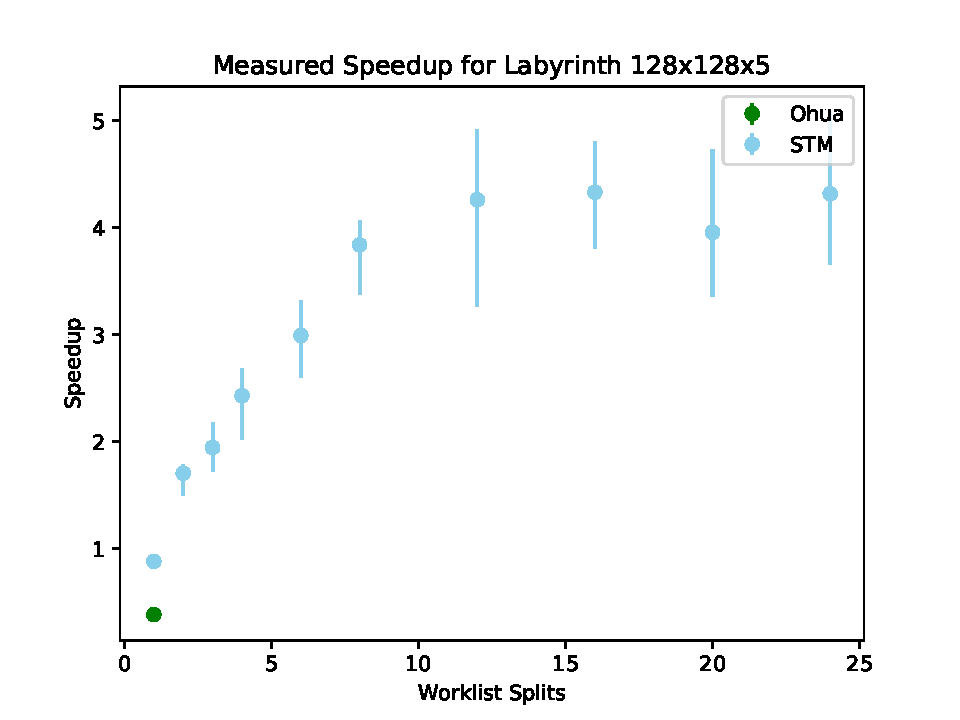
\includegraphics[width=.6\textwidth,keepaspectratio]{gfx/preliminaries-labyrinth/2019-04-18-128x128x5}
    \caption{Measured speedups of the labyrinth application for the STM and Ohua implementations.}%
    \label{fig:preliminaries:initial-results}
\end{figure}



\section{Parallel Loop Implementation}

% - present our first look into the problem that was intended to show how fit or unfit Ohua was
% - explain that we looked into "labyrinth" and show our performance
% - detail the research we did on this and what our ideas were that we explored
%   - explain how we formulated 3 optimizations to tackle the problem but don't explain them all that general but more focused on the issue at hand
%   - show effect that the optimizations had
% - show end result which validated our assumption that this could work
